% !TEX program = xelatex
\documentclass[10pt,journal,final,a4paper,nofonttune]{IEEEtran}
\usepackage[OT1]{fontenc}
\usepackage{graphicx}

\title{Demo for IEEE Journals}
\author{Yifan Yang, Liye Jia, Kai Lin, Yujie Wang}

\begin{document}
\maketitle

\begin{abstract}
    Fuck this document! This is supposed to be an abstract no shorter 
    than 100 words. However, I cannot do that myself.
\end{abstract}

\begin{IEEEkeywords}
    Fuck, Documents, No Keywords
\end{IEEEkeywords}

% \tableofcontents
% \pagebreak

\section{Introduction}
This is going to be an essay that follows the IEEE standard.
I am now writing casually without thinking what I am doing. So, the 
sentence may seem irreadable.
\cite{gomez2012overview}

This is another paragraph in the Introduction Section

Paragraph one Paragraph one Paragraph one Paragraph one Paragraph one 
Paragraph one Paragraph one Paragraph one Paragraph one Paragraph one 
Paragraph one Paragraph one Paragraph one Paragraph one Paragraph one 
Paragraph one Paragraph one Paragraph one Paragraph one Paragraph one 
Paragraph one Paragraph one Paragraph one Paragraph one Paragraph one 

Paragraph two Paragraph two Paragraph two Paragraph two Paragraph two 
Paragraph two Paragraph two Paragraph two Paragraph two Paragraph two 
Paragraph two Paragraph two Paragraph two Paragraph two Paragraph two 
Paragraph two Paragraph two Paragraph two Paragraph two Paragraph two 
Paragraph two Paragraph two Paragraph two Paragraph two Paragraph two 


\begin{figure*}[ht]
    \centering
    \begin{center}
        \caption{System Architecture}
    \end{center}
    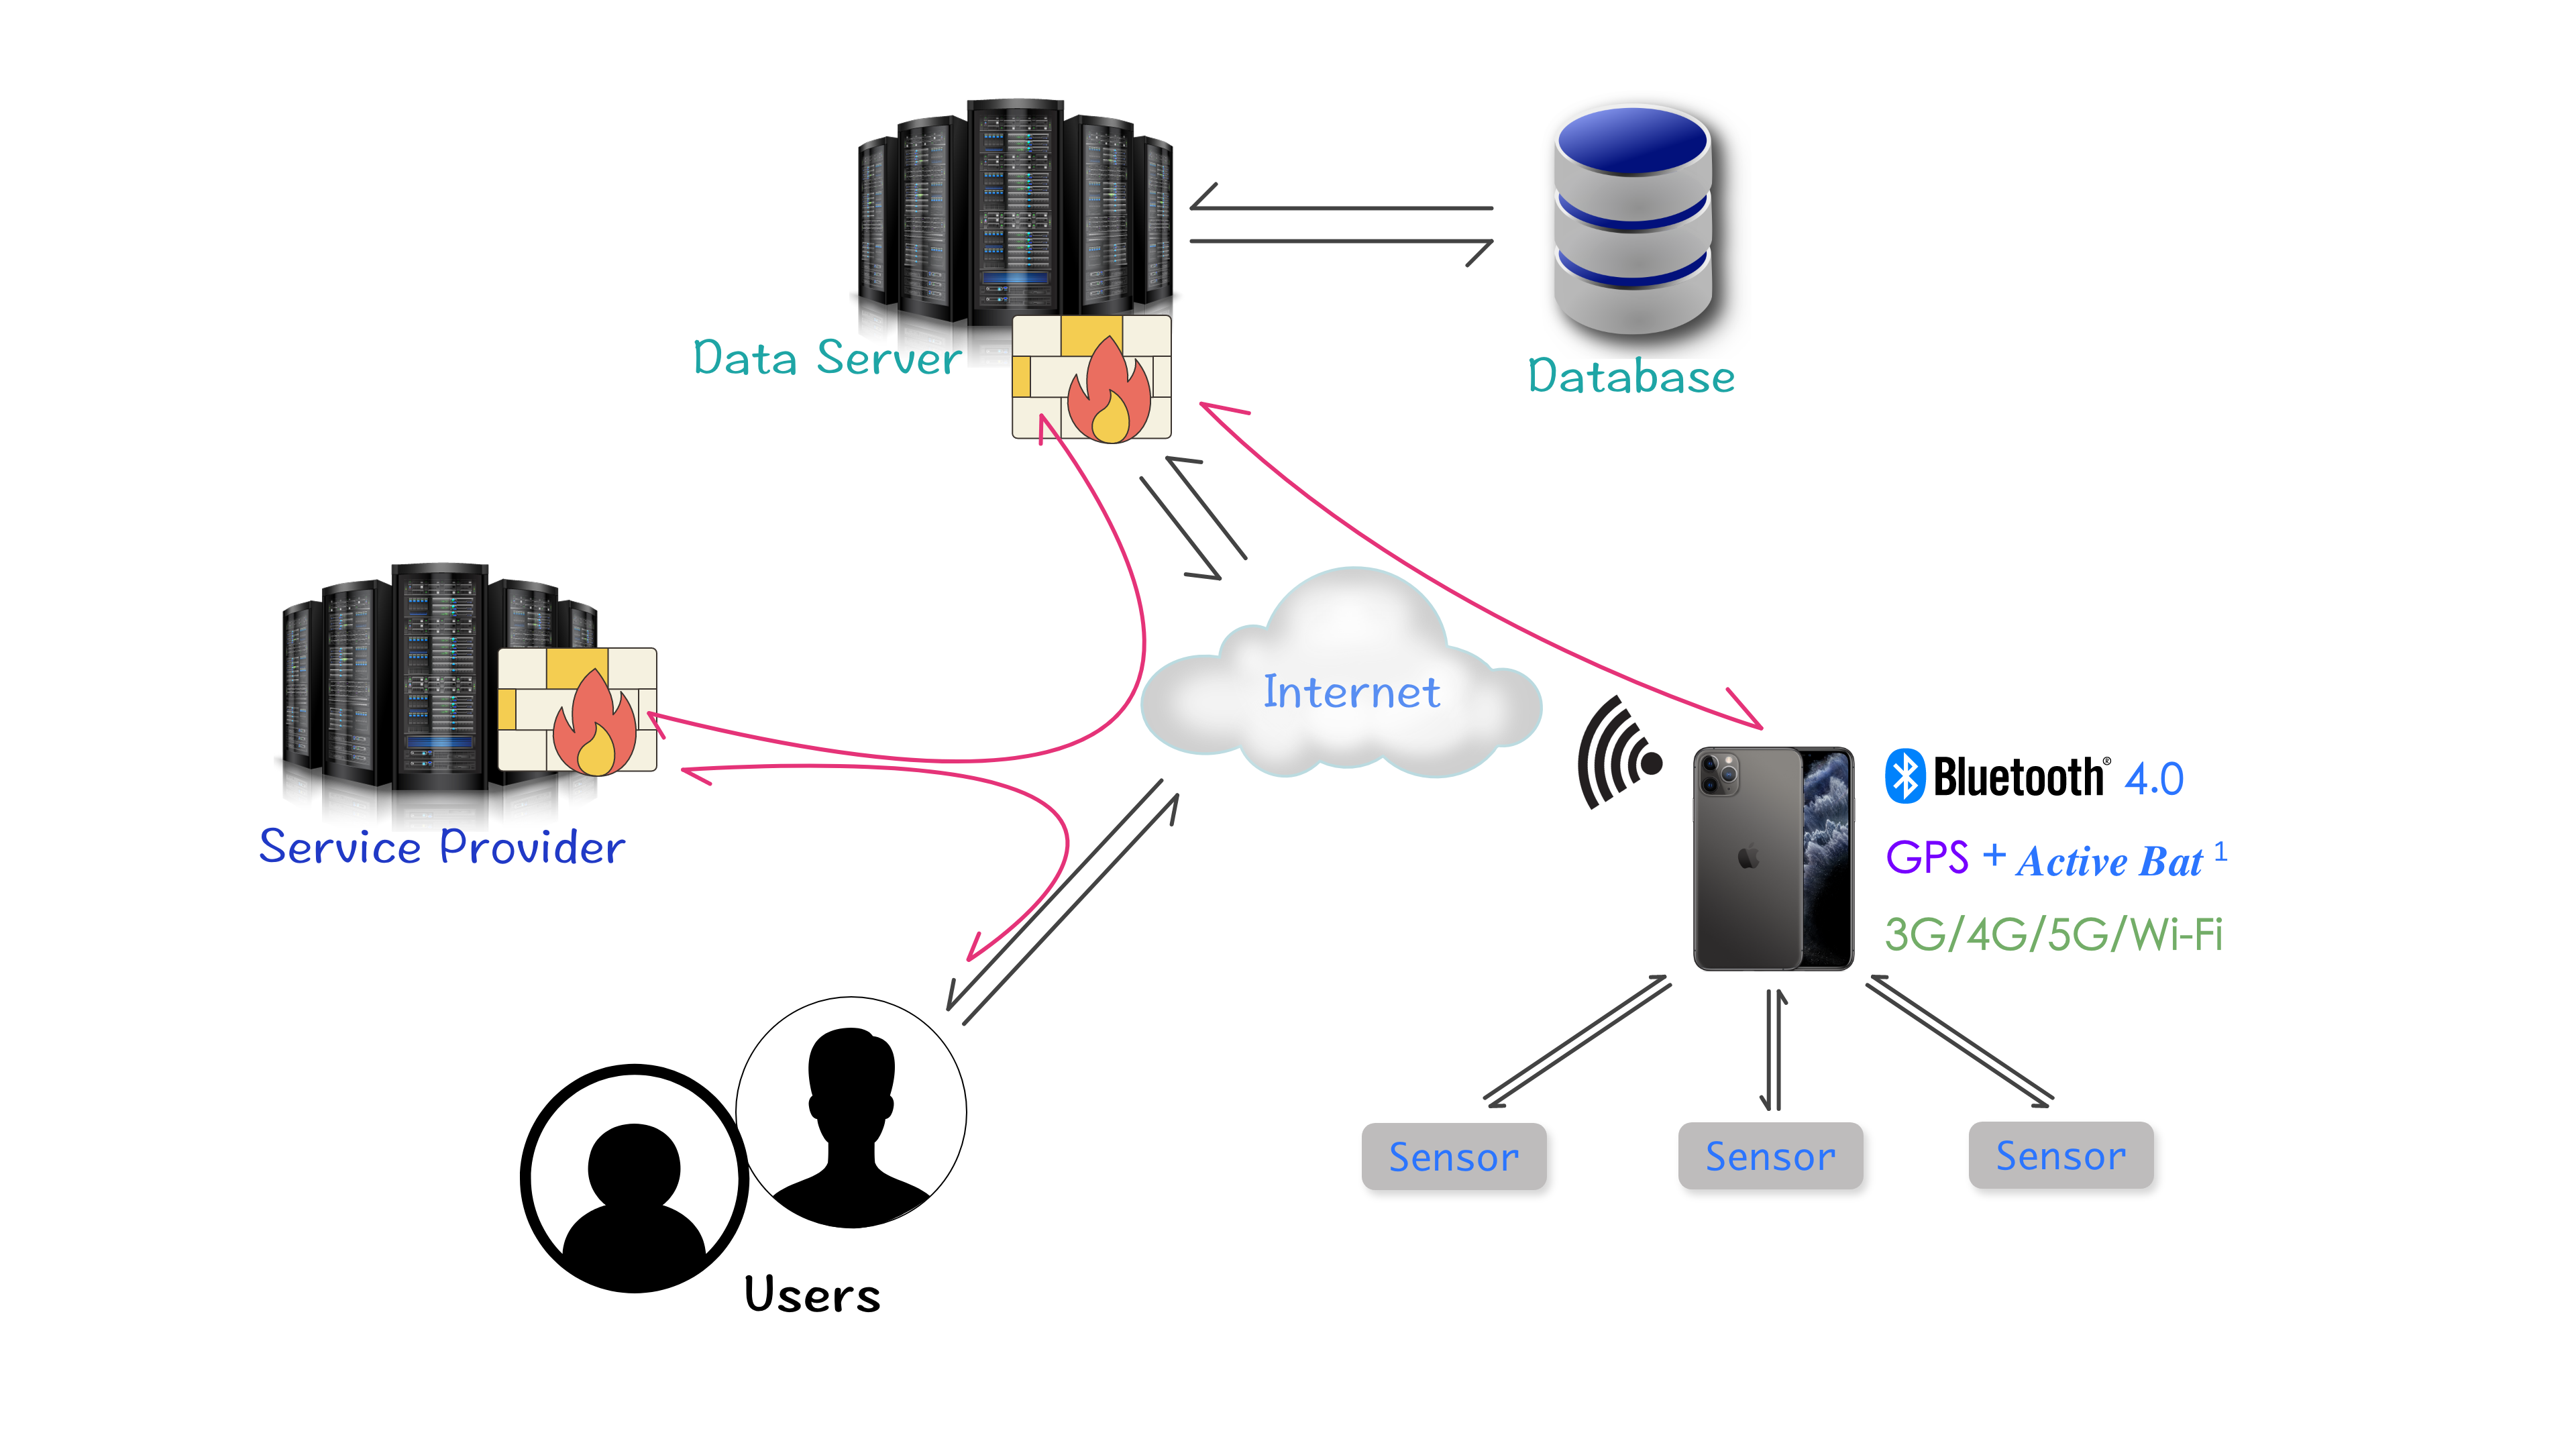
\includegraphics[width=16cm]{../Architecture.png}
\end{figure*}


\section{System Description}

\subsection{Hardware}

\subsubsection{Location System}
\subsubsection{Sensors} 

content

\begin{table}[h]
    % \Large
    \caption{Sample Table}
    \begin{center}
        \begin{tabular}{|p{1cm}|p{2cm}|p{1cm}|p{2cm}|}
            \hline
            Sensors & Energy Consumption & Accuracy & Description \\ \hline
            Blood Pressure & 50mW & ~2\% & This Description should be displays in multiple lines if it is this long. \\ 
            \hline
        \end{tabular}
    \end{center}
\end{table}


\subsection{Network}

\begin{figure}[!ht]
    \centering
    \begin{center}
        \caption{System Architecture}
    \end{center}
    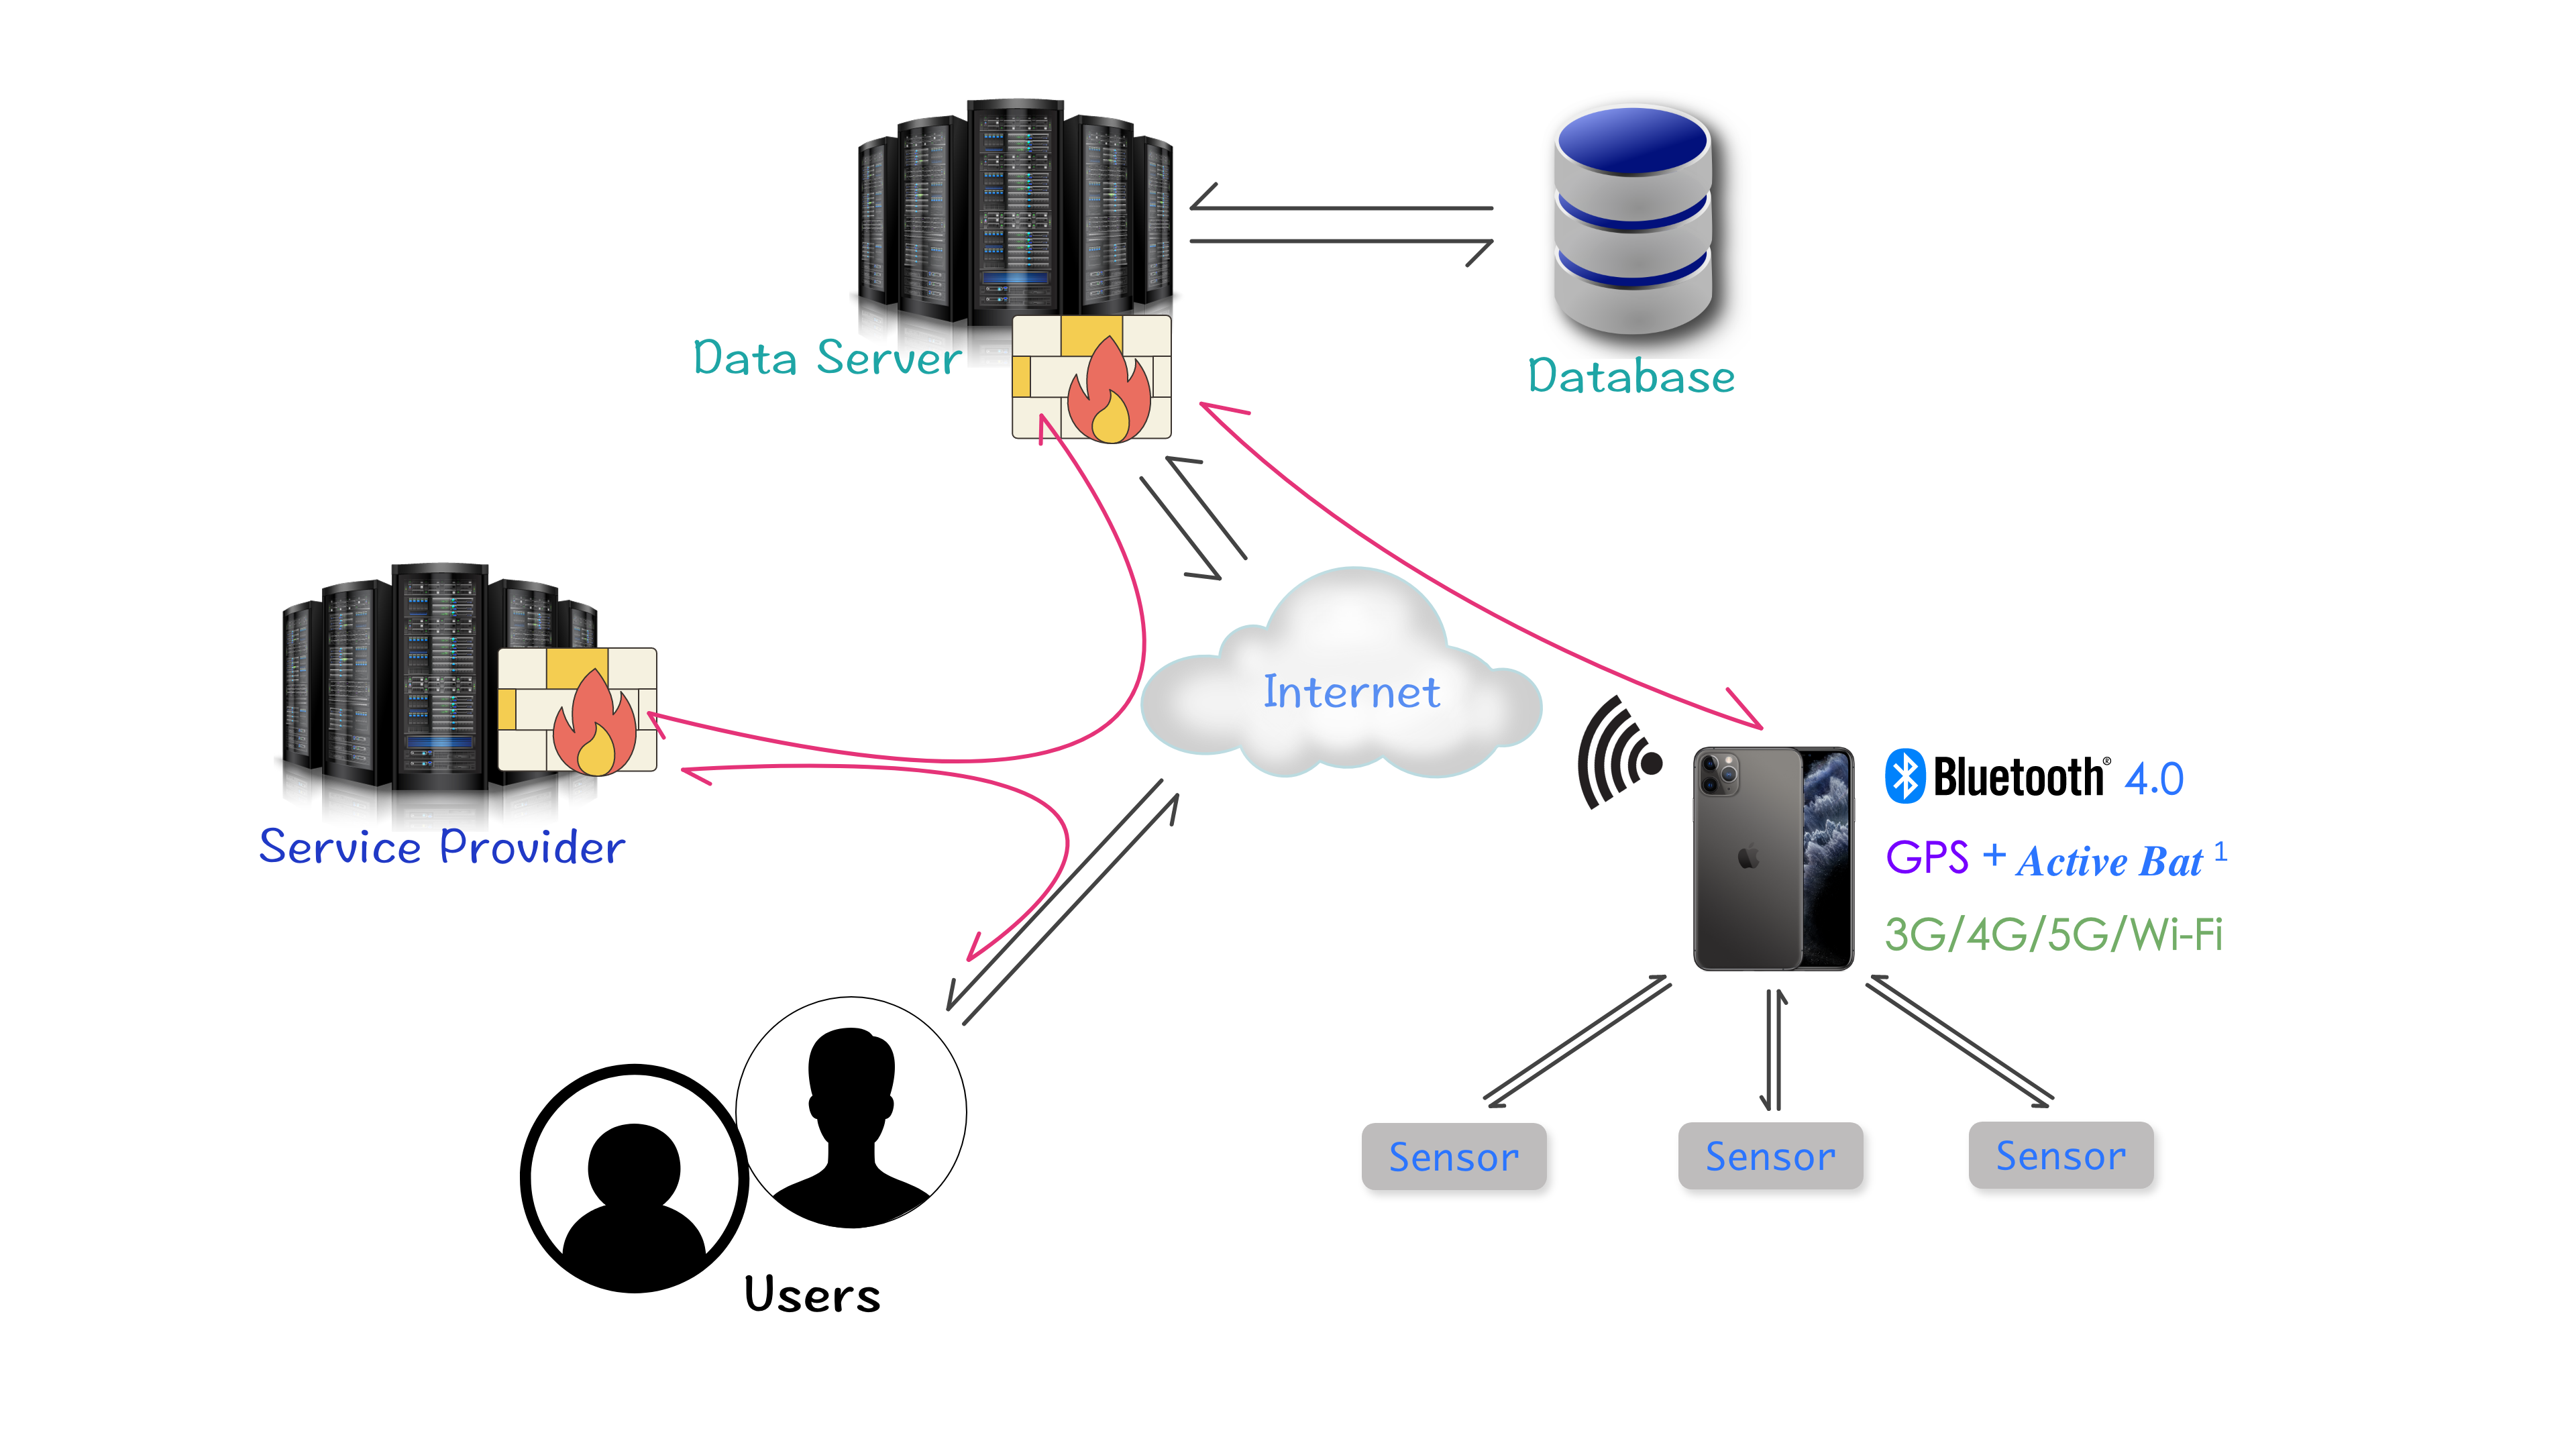
\includegraphics[width=8cm]{../Architecture.png}
\end{figure}

Paragraph two Paragraph two Paragraph two Paragraph two Paragraph two 
Paragraph two Paragraph two Paragraph two Paragraph two Paragraph two 
Paragraph two Paragraph two Paragraph two Paragraph two Paragraph two 
Paragraph two Paragraph two Paragraph two Paragraph two Paragraph two 
Paragraph two Paragraph two Paragraph two Paragraph two Paragraph two 

\subsection{Internet Data Flow}


udbcsiuhcbaiuejwndfciujwds


\subsection{Application Layer}


\subsubsection{Cloud Computing and Database}

\subsubsection{Other Concerns}


\section{Use Case Scenarios}
Paragraph one Paragraph one Paragraph one Paragraph one Paragraph one 
Paragraph one Paragraph one Paragraph one Paragraph one Paragraph one 
Paragraph one Paragraph one Paragraph one Paragraph one Paragraph one 
Paragraph one Paragraph one Paragraph one Paragraph one Paragraph one 
Paragraph one Paragraph one Paragraph one Paragraph one Paragraph one 

Paragraph two Paragraph two Paragraph two Paragraph two Paragraph two 
Paragraph two Paragraph two Paragraph two Paragraph two Paragraph two 
Paragraph two Paragraph two Paragraph two Paragraph two Paragraph two 
Paragraph two Paragraph two Paragraph two Paragraph two Paragraph two 
Paragraph two Paragraph two Paragraph two Paragraph two Paragraph two 

\section{Conclusion}

Paragraph one Paragraph one Paragraph one Paragraph one Paragraph one 
Paragraph one Paragraph one Paragraph one Paragraph one Paragraph one 
Paragraph one Paragraph one Paragraph one Paragraph one Paragraph one 
Paragraph one Paragraph one Paragraph one Paragraph one Paragraph one 
Paragraph one Paragraph one Paragraph one Paragraph one Paragraph one 

Paragraph two Paragraph two Paragraph two Paragraph two Paragraph two 
Paragraph two Paragraph two Paragraph two Paragraph two Paragraph two 
Paragraph two Paragraph two Paragraph two Paragraph two Paragraph two 
Paragraph two Paragraph two Paragraph two Paragraph two Paragraph two 
Paragraph two Paragraph two Paragraph two Paragraph two Paragraph two 

\section*{Acknowledgments}

Paragraph one Paragraph one Paragraph one Paragraph one Paragraph one 
Paragraph one Paragraph one Paragraph one Paragraph one Paragraph one 
Paragraph one Paragraph one Paragraph one Paragraph one Paragraph one 
Paragraph one Paragraph one Paragraph one Paragraph one Paragraph one 
Paragraph one Paragraph one Paragraph one Paragraph one Paragraph one 

Paragraph three

\bibliographystyle{IEEEtran}
\bibliography{References}
\end{document}